\documentclass[a4paper, 12pt]{article}

\def\languages{french, english}

%%%%%%%%%%%%%%%%%%% Libraries

\input{include/libraries/bibliography.tex}
\input{include/libraries/default.tex}
\input{include/libraries/figures.tex}
\input{include/libraries/informatics.tex}
\input{include/libraries/mathematics.tex}
\input{include/libraries/theorems.tex}
\input{include/libraries/units.tex}

\input{include/languages/french.tex}

%%%%%%%%%%%%%%%%%%% Titlepage

\def\logopath{resources/pdf/logo-uliege.pdf}
\def\toptitle{University of Liège}
\title{Homework 3}
\def\subtitle{Applied digital signal processing}
%\def\authorhead{Author}
\author{
    Quentin \textsc{Graillet} (20164386)\\
    Maxime \textsc{Meurisse} (20161278)\\
    Adrien \textsc{Schoffeniels} (20162843)\\
}
%\def\rightauthorhead{}
%\def\rightauthor{}
\def\context{3\ieme{} year of Bachelor Civil Engineer}
\date{Academic year 2018-2019}

%%%%%%%%%%%%%%%%%%%

\fancyhead[R]{}
\NFstyle{matlab}

%%%%%%%%%%%%%%%%%%%

\begin{document}
	\input{include/titlepages/default.tex}
	\section*{Noise filtering}
	We have a noisy signal
	\begin{equation*}
	    x_{\text{ns}}[n] = x[n] + v[n]
	\end{equation*}
	where
	\begin{equation*}
	    x[n] = \cos(20\pi t) + \num{0.5}\cos(40\pi t + \num{1.4}) + \num{0.8}\cos(120\pi t + \num{0.7})
	\end{equation*}
	and $v[n]$ is an arbitrary noise.\par
	Signals $x_{\text{ns}}[n]$ and $x[n]$ are sampled at \SI{1000}{\hertz}.\par
	The goal is to design a filter to remove the noise from $x_{\text{ns}}[n]$ without distortion.
	\subsection*{Question a}
	We plot signals $x[n]$ and $x_{\text{ns}}[n]$ in the same axis (figure \ref{fig:question_a}).
	\begin{figure}[H]
	    \centering
	    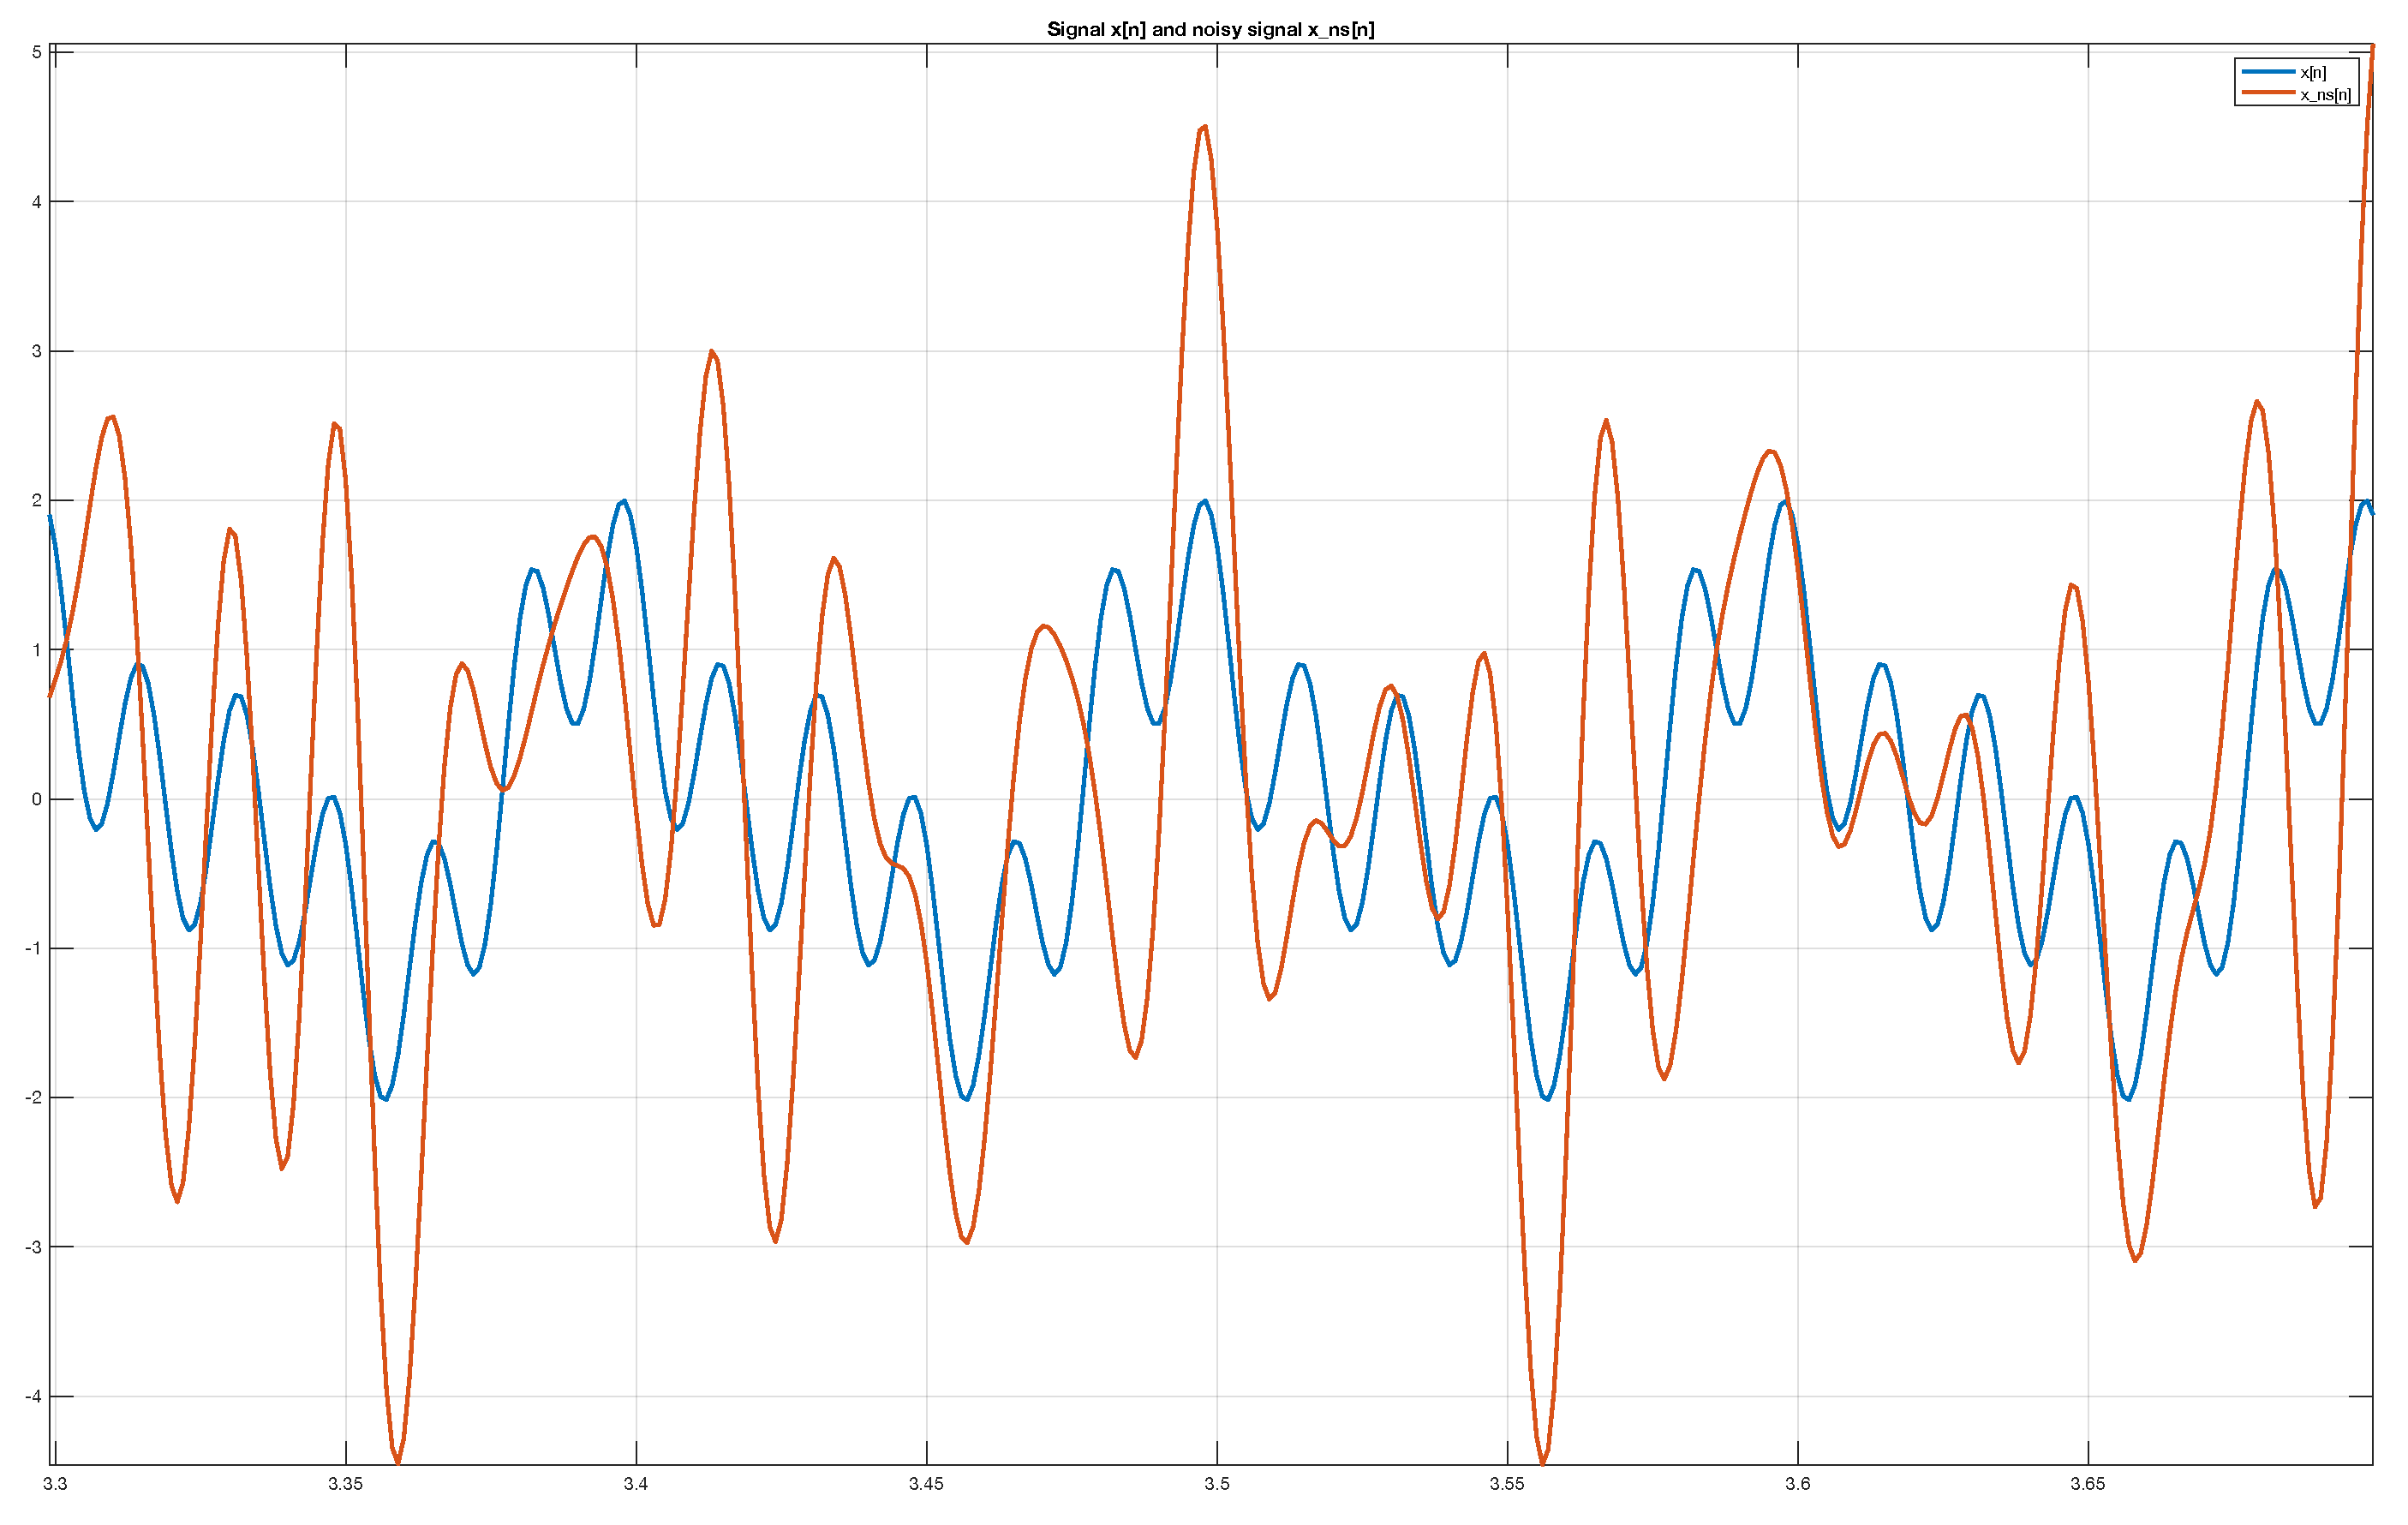
\includegraphics[width=\textwidth]{resources/pdf/question_a.pdf}
	    \caption{Signals $x[n]$ and $x_{\text{ns}}[n]$ in the same axis.}
	    \label{fig:question_a}
	\end{figure}
	\subsection*{Question b}
	We plot the single-sided amplitude spectrum of the noisy signal $x_{\text{ns}}[n]$ (figure \ref{fig:question_b}).
	\begin{figure}[H]
	    \centering
	    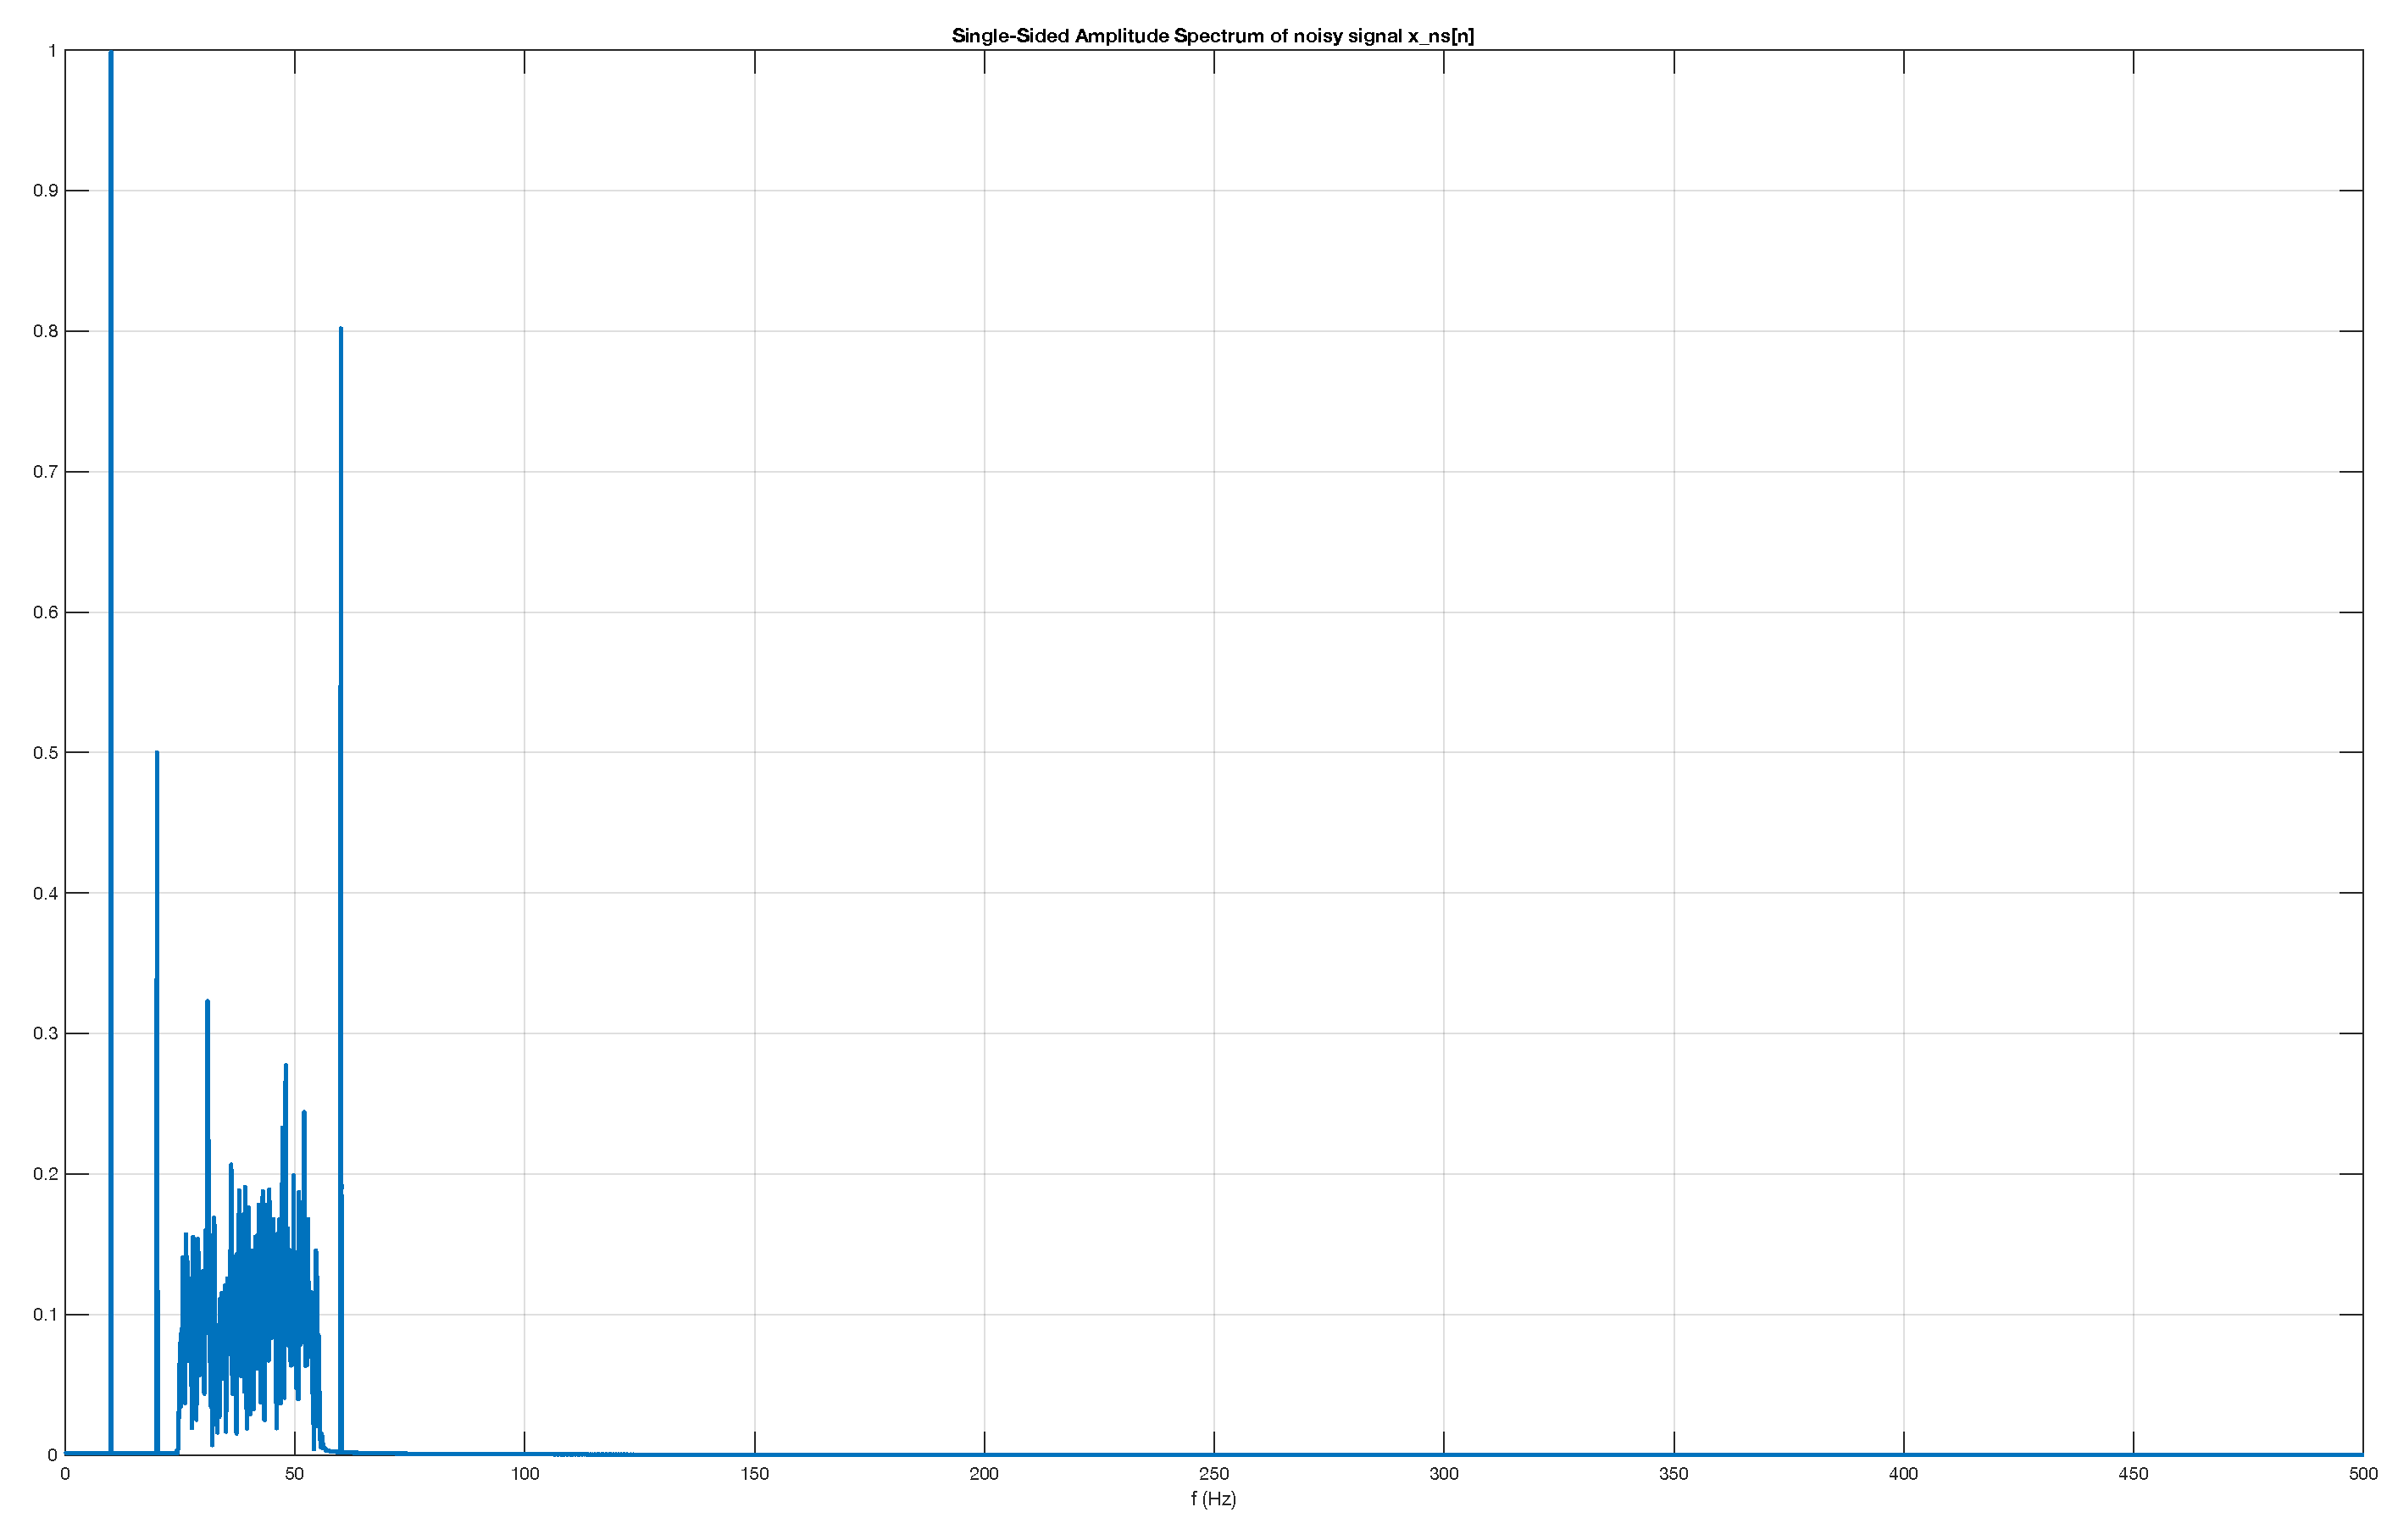
\includegraphics[width=\textwidth]{resources/pdf/question_b.pdf}
	    \caption{Single-sided amplitude spectrum of the noisy signal $x_{\text{ns}}[n]$.}
	    \label{fig:question_b}
	\end{figure}
	\subsection*{Question c}
	Thanks to the figure \ref{fig:question_b} and a piece of code, we determined that the approximate frequency range of the noise $v[n]$ is $[24, 56]$ [Hz].
	\subsection*{Question d}
	As we want to preserve the shape of the signal, we have to design an \emph{FIR} filter.\par
	Thanks to Matlab, we can create such a filter easily. Properties of the created filter are presented at figure \ref{fig:question_d}.
	\begin{figure}[H]
	    \centering
	    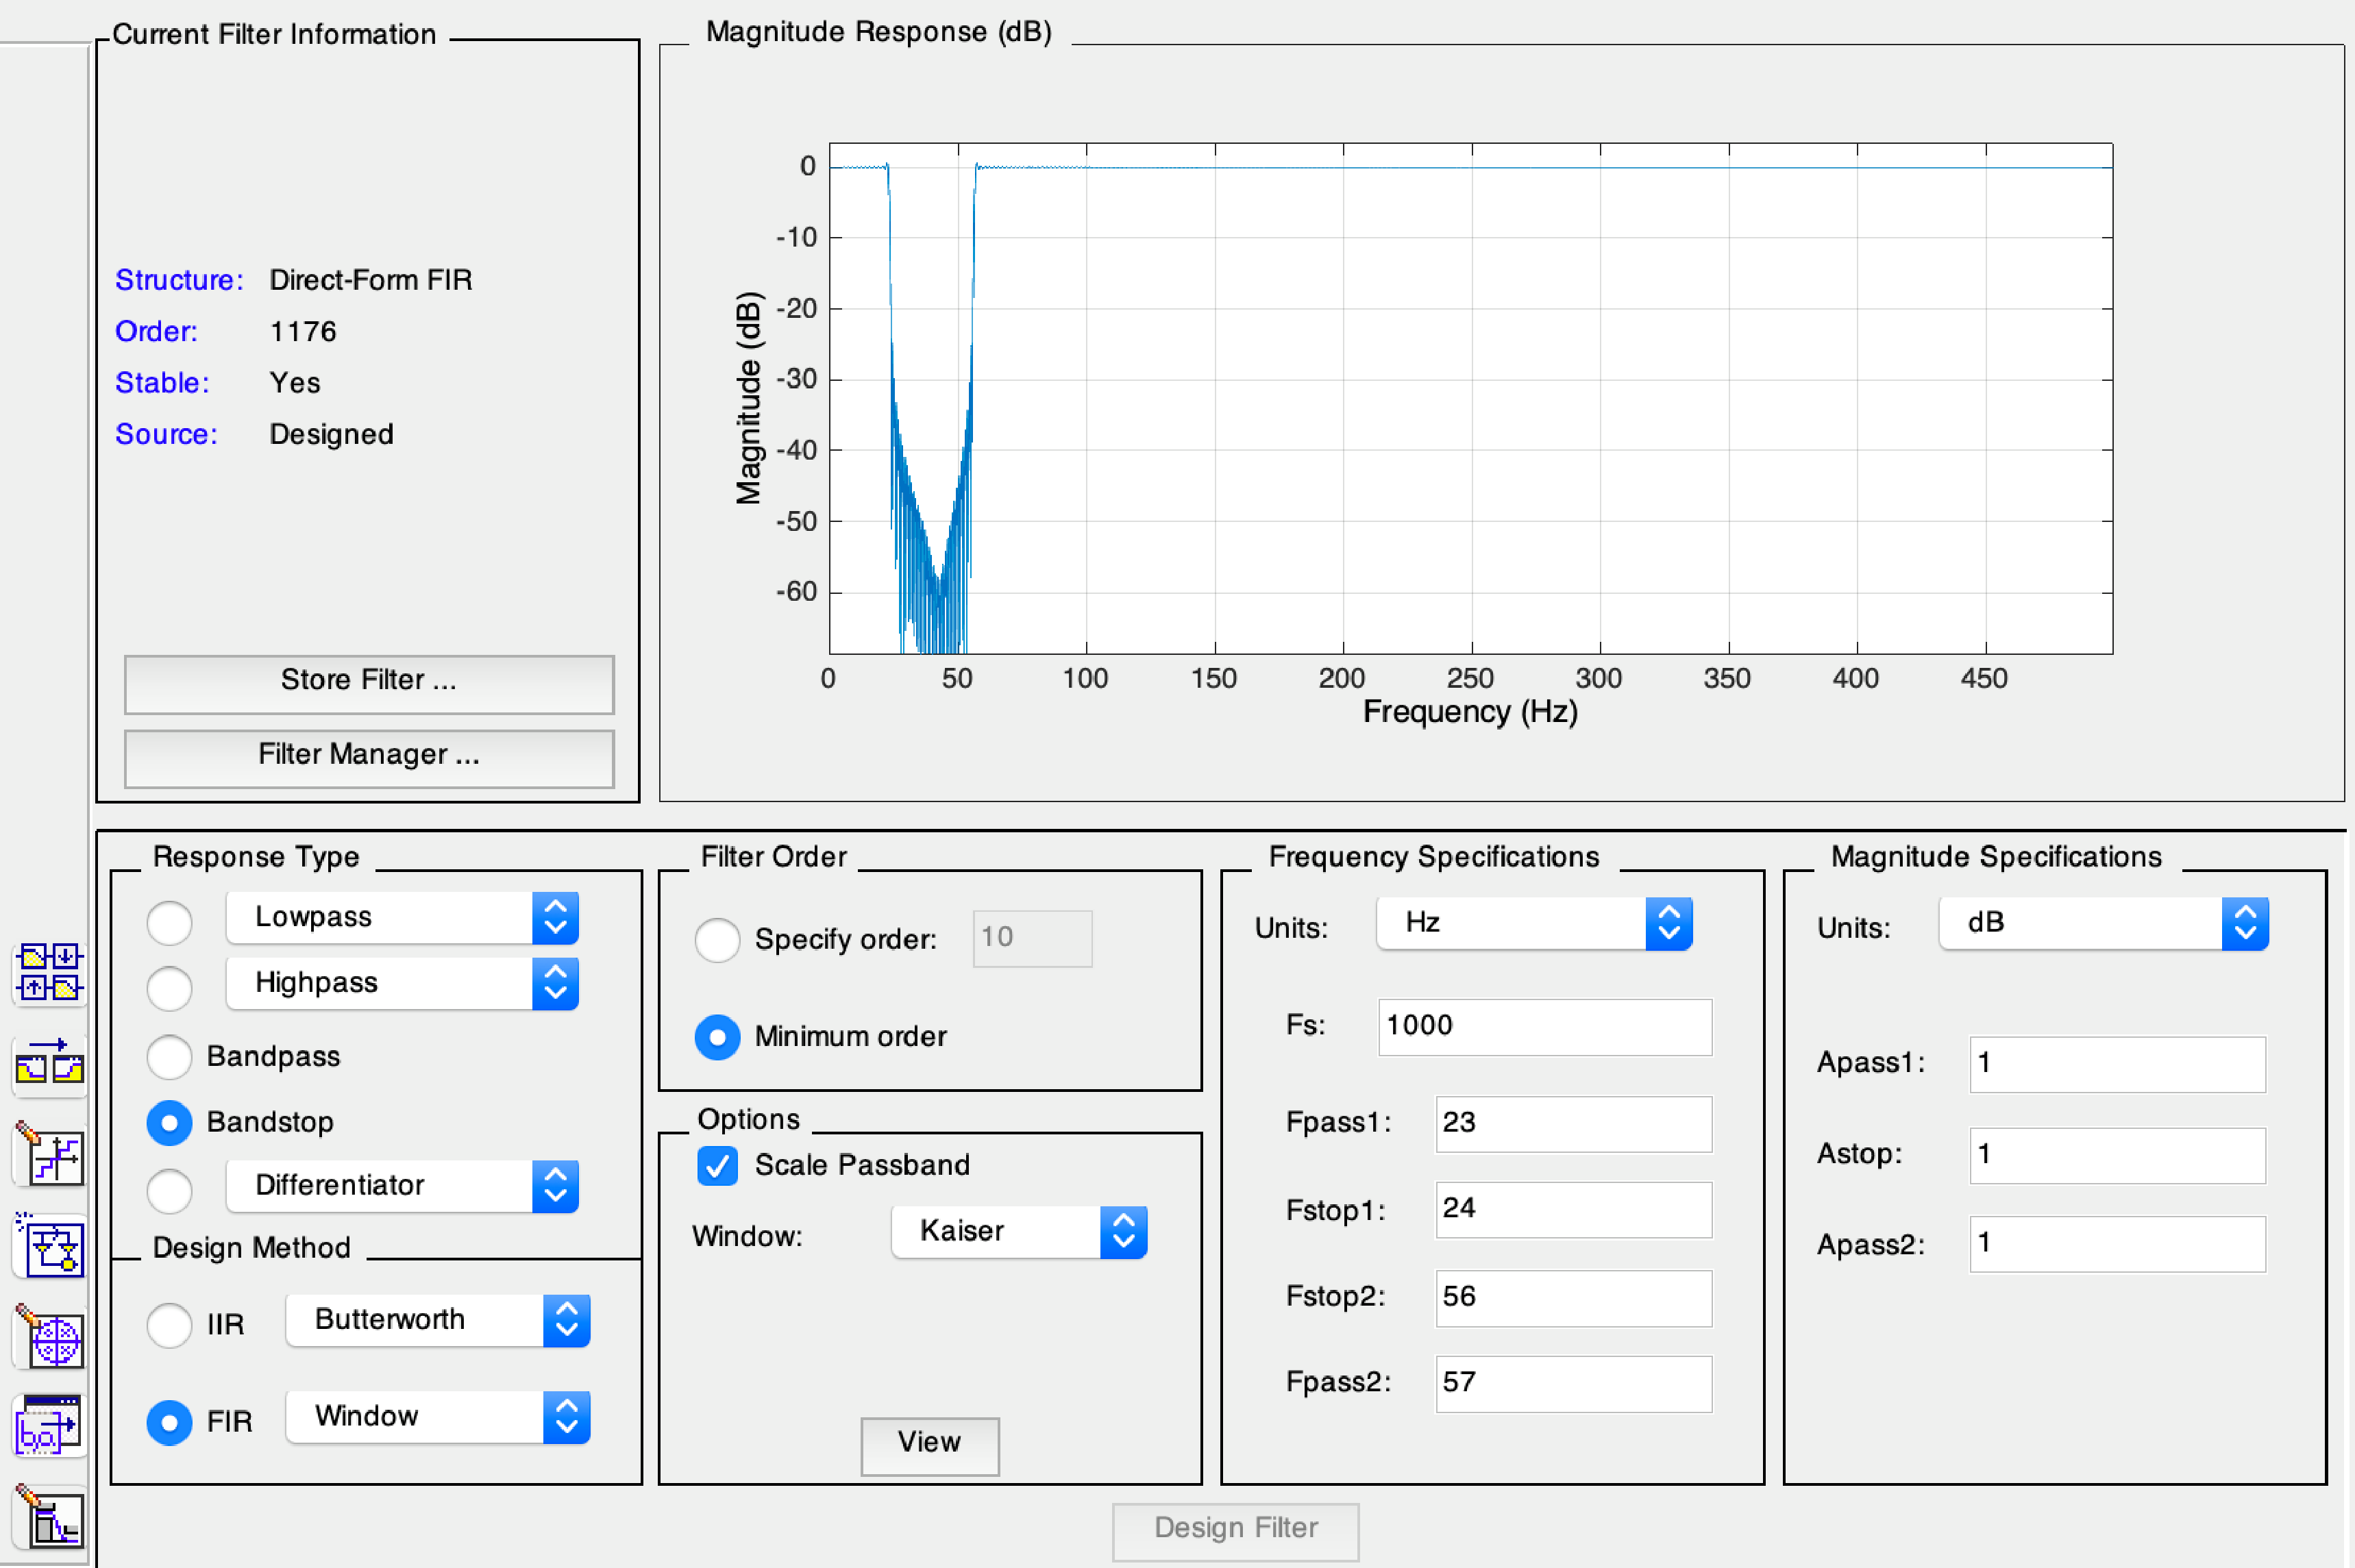
\includegraphics[width=\textwidth]{resources/pdf/question_d.pdf}
	    \caption{Design of the \emph{FIR} filter.}
	    \label{fig:question_d}
	\end{figure}
	So, we choose a \emph{FIR} filter in the options. We set $F_s$ to \SI{1000}{\hertz}, and $F_\text{stop1}$ and $F_\text{stop2}$ respectively to \num{24} and \SI{56}{\hertz}. We also set $A_\text{stop}$ to \SI{1}{\deci\bel}.
	\subsection*{Question e}
	After applying the filter on the noisy signal, we plot the single-sided amplitude spectrum of the filtered signal $x_\text{filt}[n]$ (figure \ref{fig:question_e}).
	\begin{figure}[H]
	    \centering
	    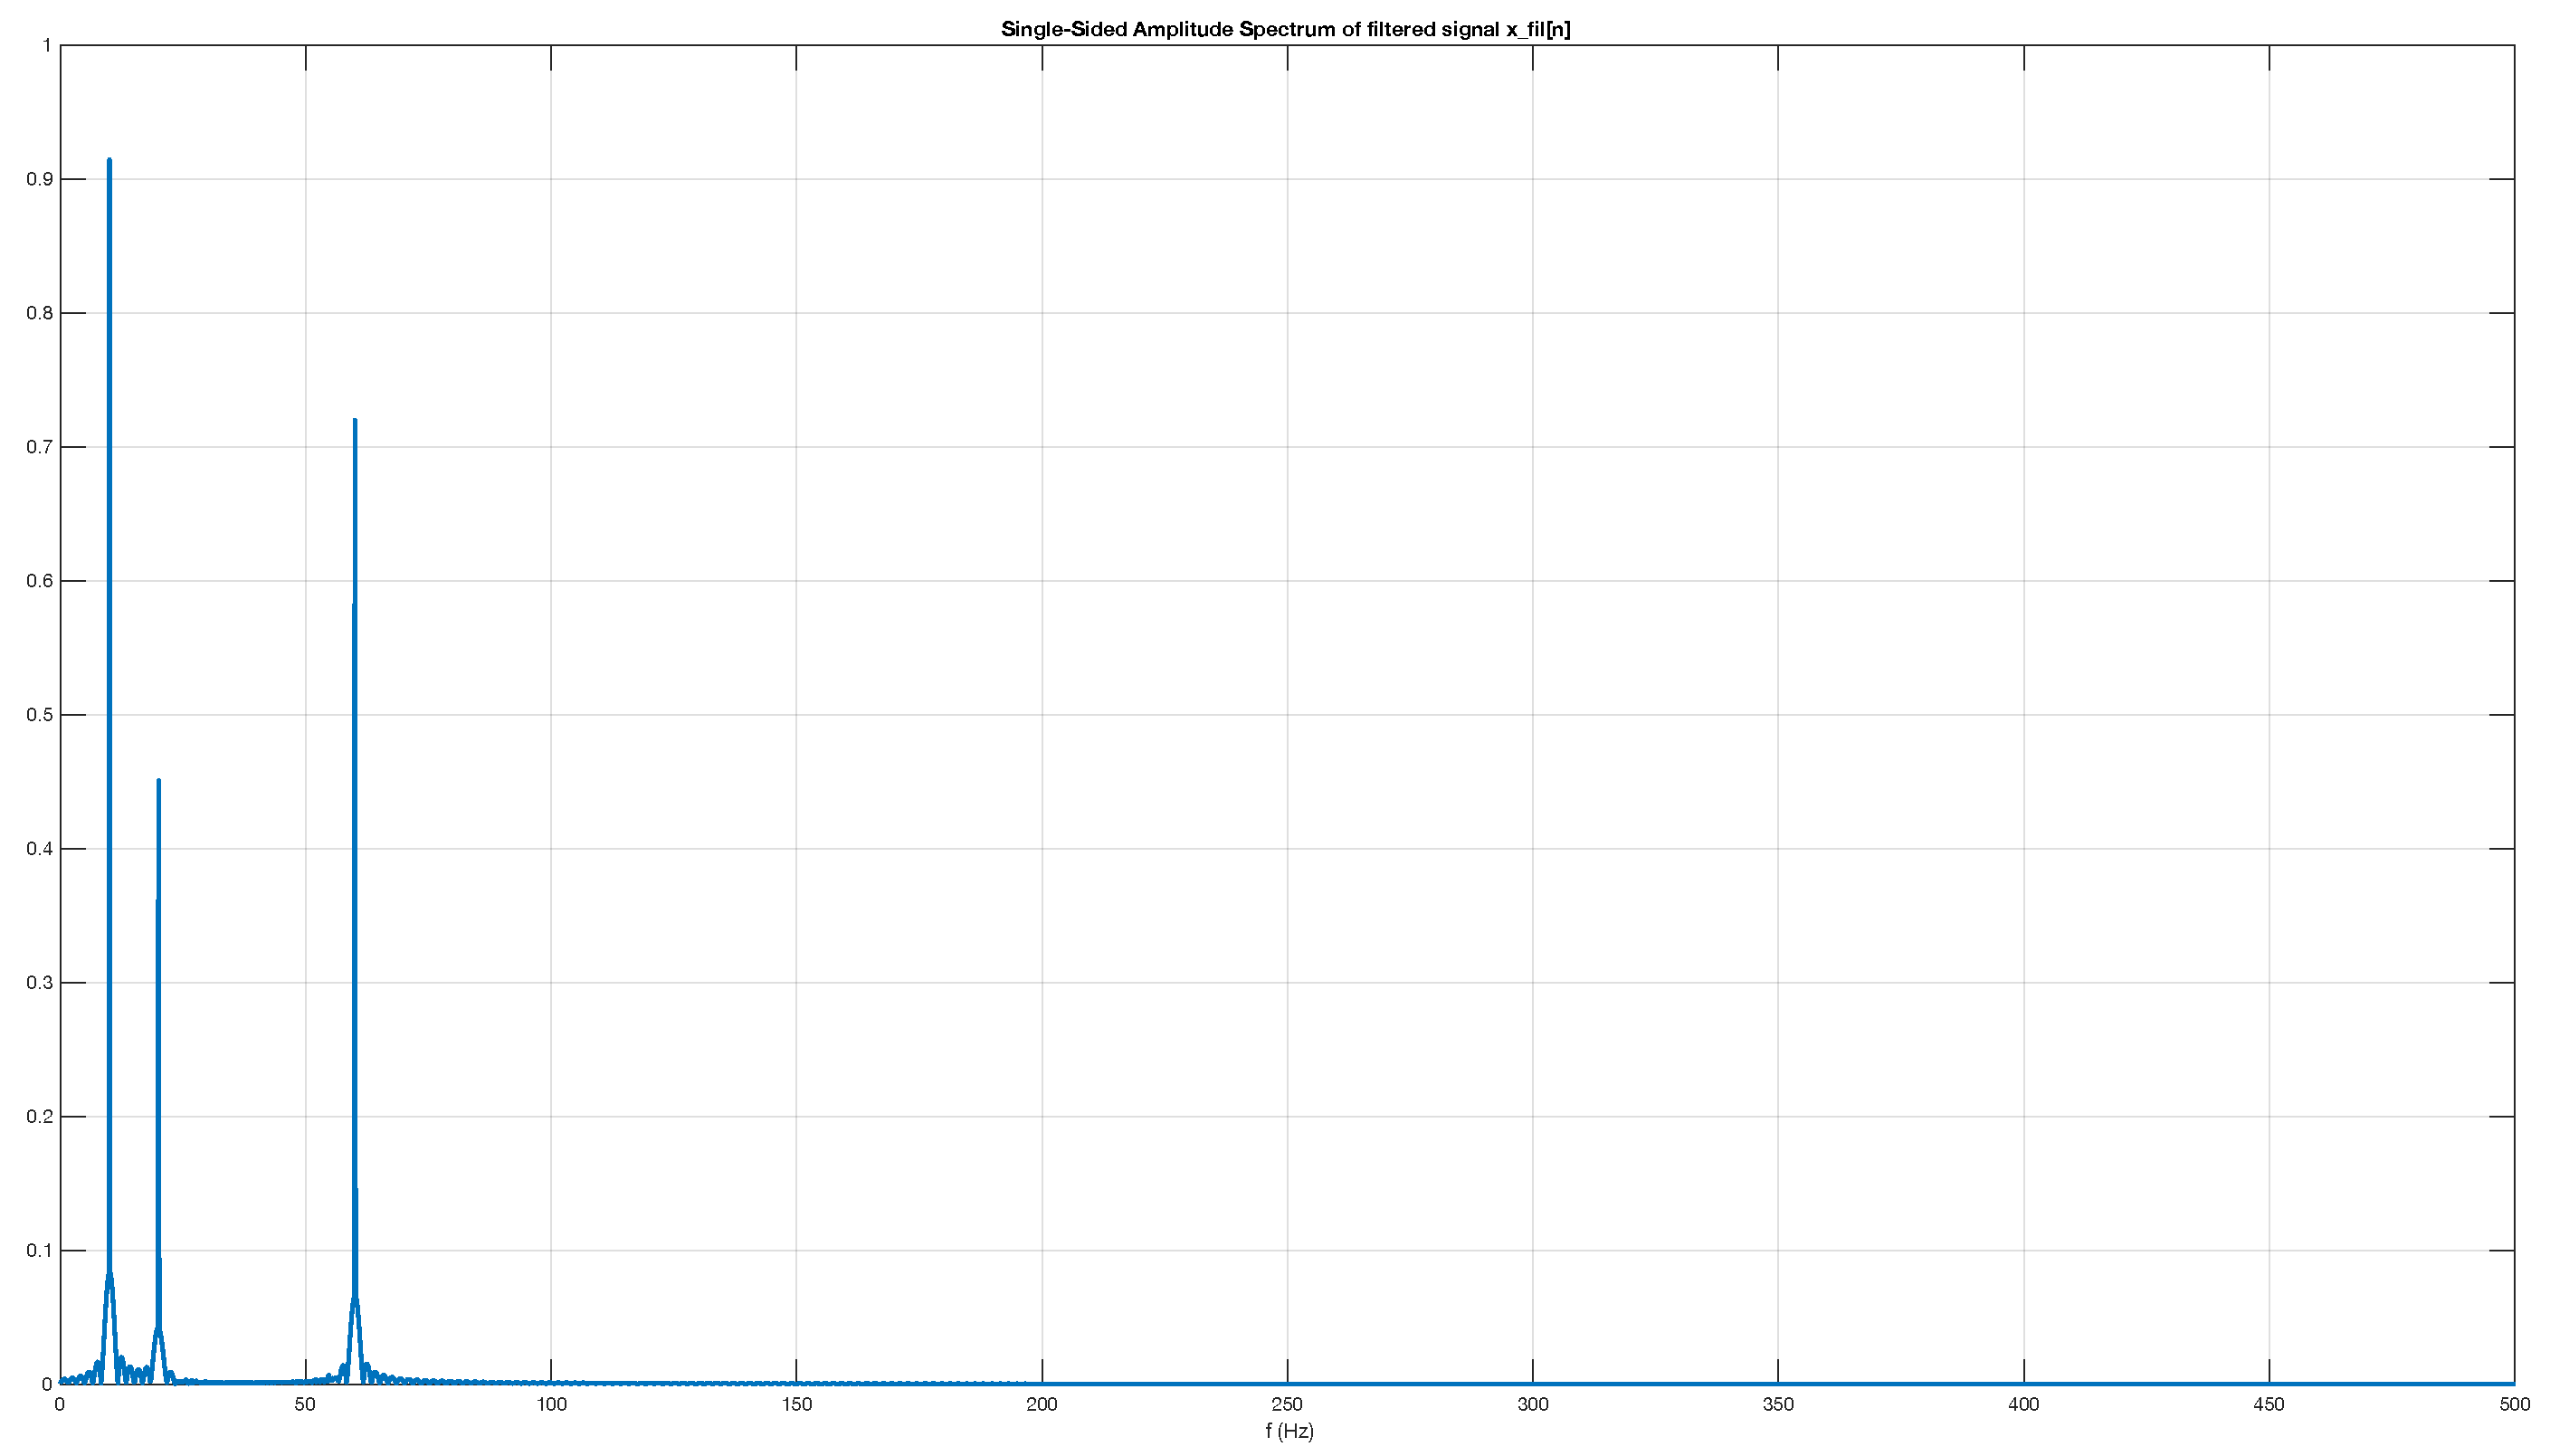
\includegraphics[width=\textwidth]{resources/pdf/question_e.pdf}
	    \caption{Single-sided amplitude spectrum of the filtered signal $x_\text{filt}[n]$.}
	    \label{fig:question_e}
	\end{figure}
	We clearly see that the noise in the frequency range $[24, 56]$ [Hz] has been attenuated.
	\subsection*{Question f}
	Finally, we plot signals $x[n]$ and $x_\text{fil}[n]$ in the same axis to check the result of our \emph{FIR} filter (figure \ref{fig:question_f}).
	\begin{figure}[H]
	    \centering
	    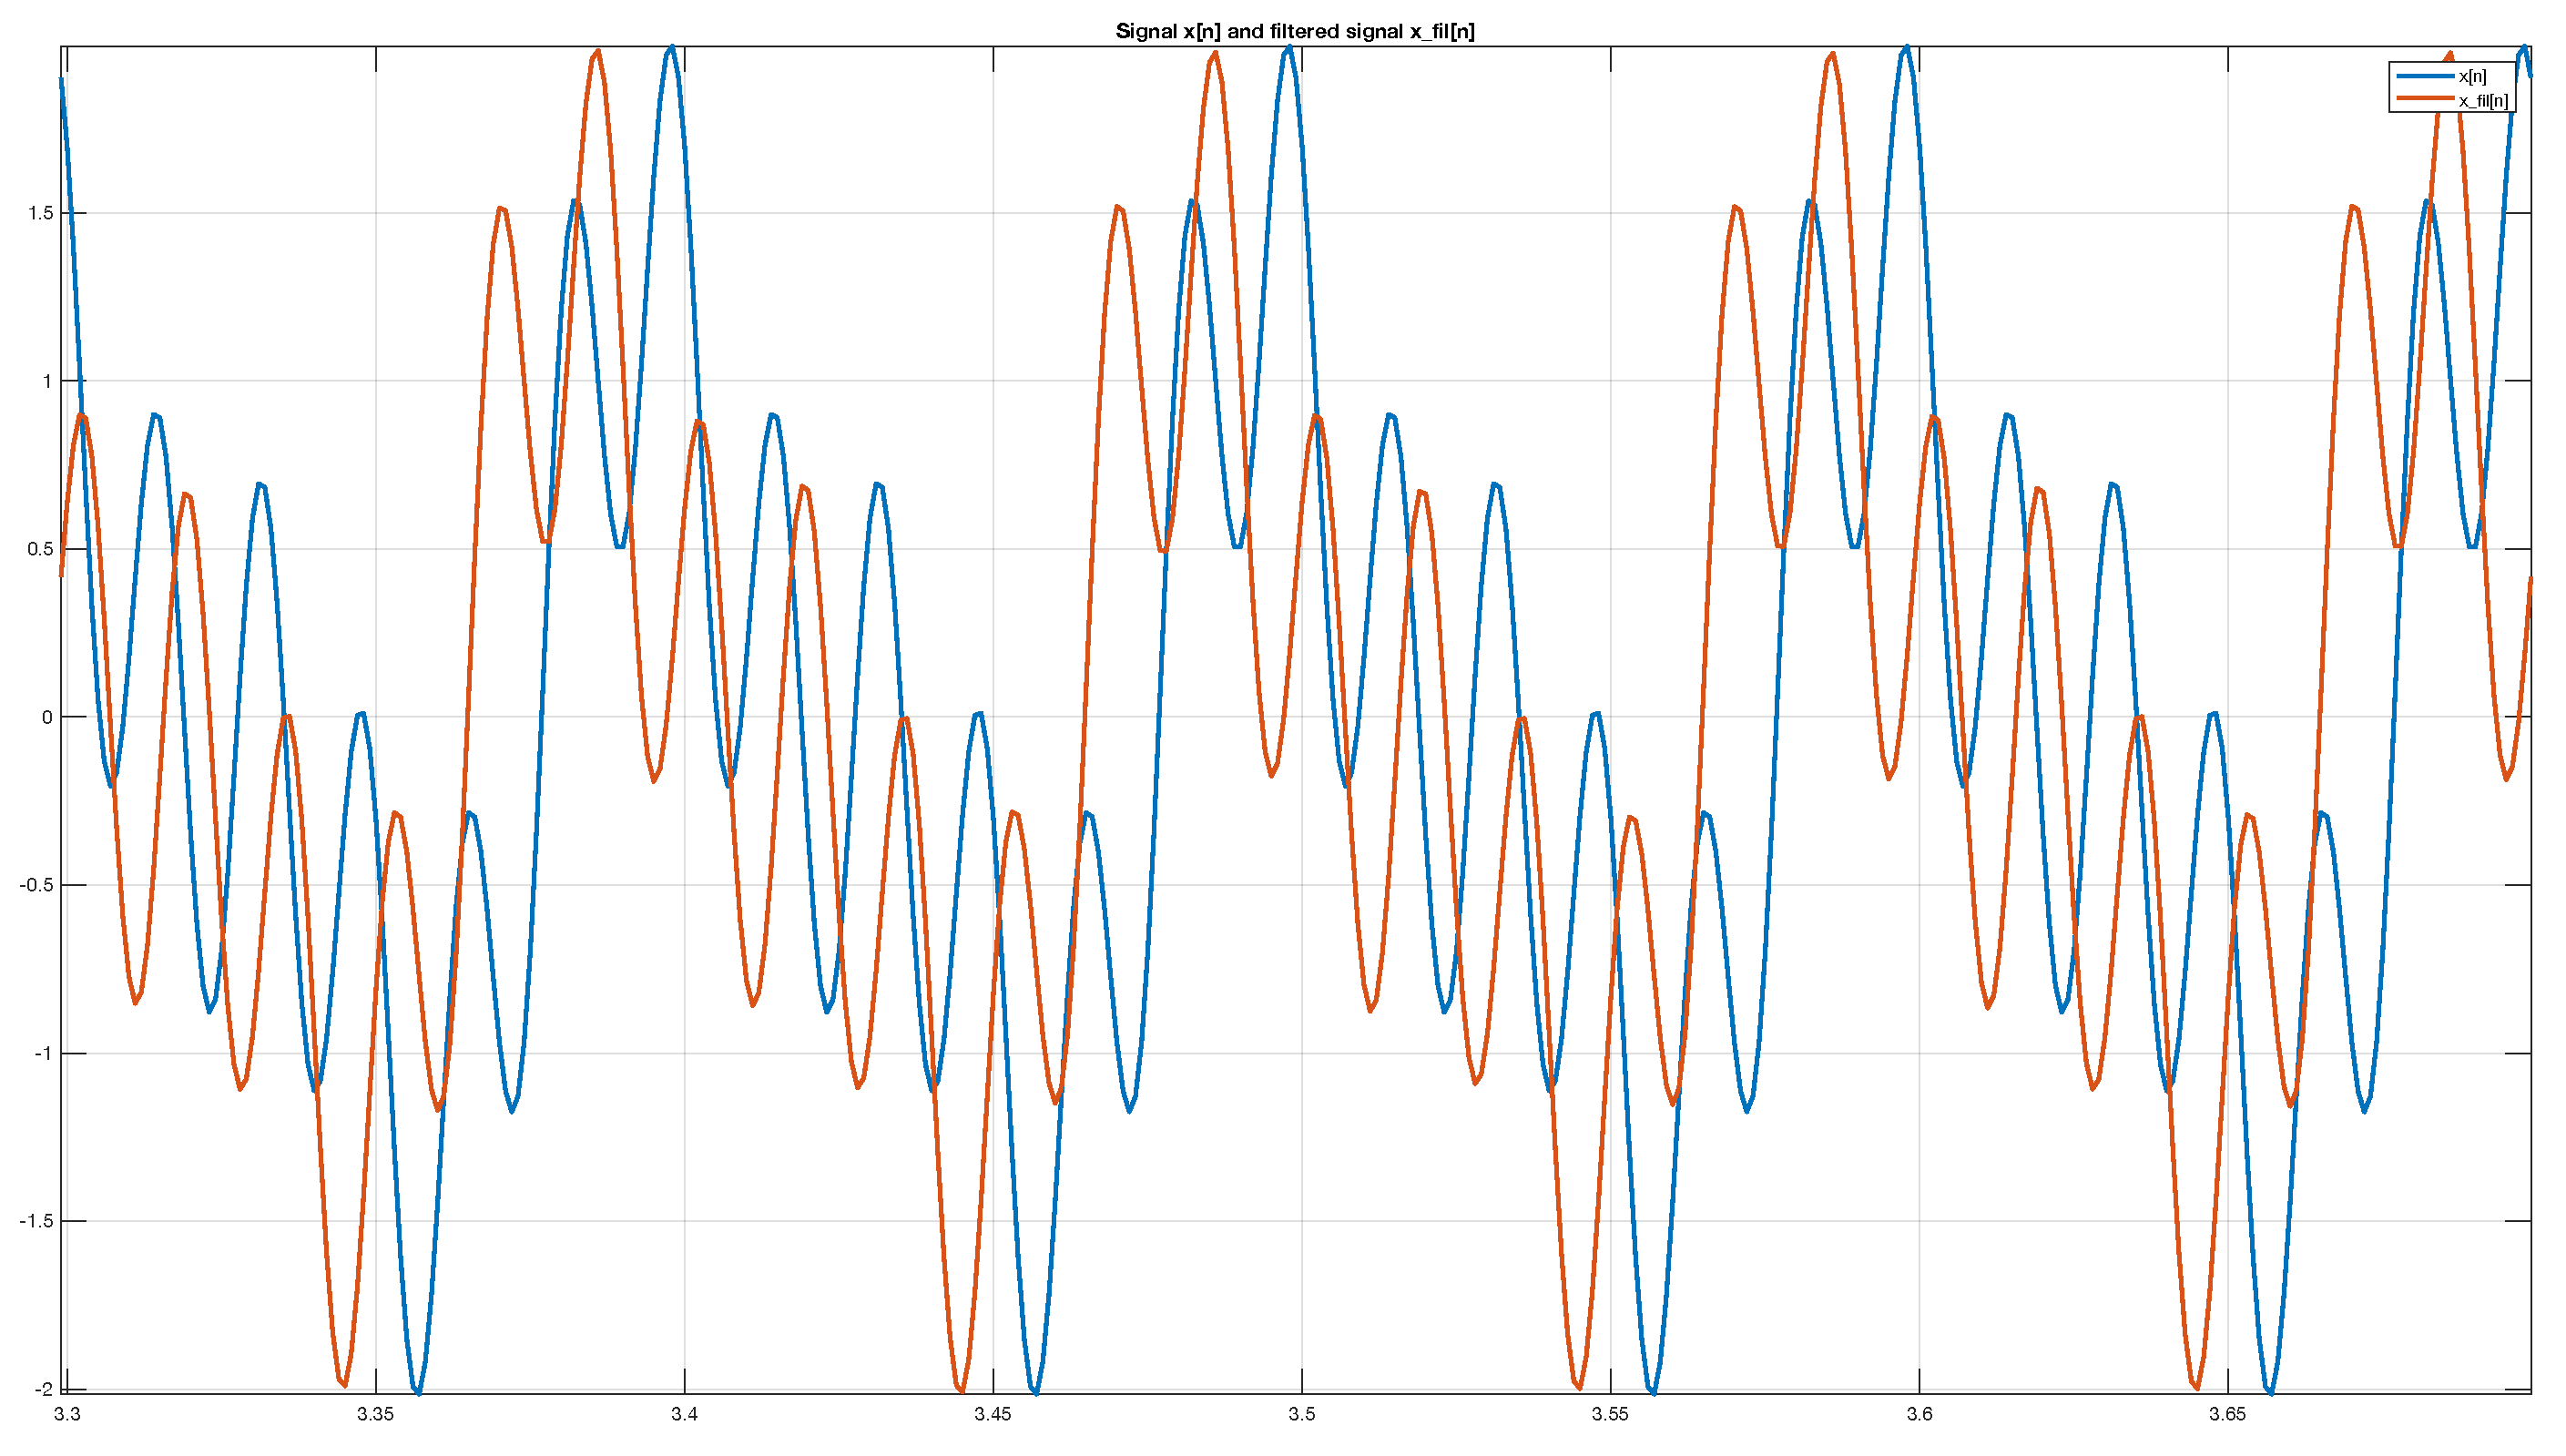
\includegraphics[width=\textwidth]{resources/pdf/question_f.pdf}
	    \caption{Signals $x[n]$ and $x_\text{fil}[n]$ in the same axis.}
	    \label{fig:question_f}
	\end{figure}
	We can observe that the signal $x_\text{fil}[n]$ is exactly the same than the original signal $x[n]$ (no distortion occurred because \emph{FIR} filter has linear phase response).
	\newpage
	\appendix
	\section*{Matlab code}
	\lstinputlisting[style=NFmatlab]{resources/m/Q1.m}
\end{document}
